% interactcadsample.tex
% v1.03 - April 2017

\documentclass[]{interact}

\usepackage{epstopdf}% To incorporate .eps illustrations using PDFLaTeX, etc.
\usepackage{subfigure}% Support for small, `sub' figures and tables
%\usepackage[nolists,tablesfirst]{endfloat}% To `separate' figures and tables from text if required

\usepackage{natbib}% Citation support using natbib.sty
\bibpunct[, ]{(}{)}{;}{a}{}{,}% Citation support using natbib.sty
\renewcommand\bibfont{\fontsize{10}{12}\selectfont}% Bibliography support using natbib.sty

\theoremstyle{plain}% Theorem-like structures provided by amsthm.sty
\newtheorem{theorem}{Theorem}[section]
\newtheorem{lemma}[theorem]{Lemma}
\newtheorem{corollary}[theorem]{Corollary}
\newtheorem{proposition}[theorem]{Proposition}

\theoremstyle{definition}
\newtheorem{definition}[theorem]{Definition}
\newtheorem{example}[theorem]{Example}

\theoremstyle{remark}
\newtheorem{remark}{Remark}
\newtheorem{notation}{Notation}

% see https://stackoverflow.com/a/47122900
\usepackage{color}
\usepackage{fancyvrb}
\newcommand{\VerbBar}{|}
\newcommand{\VERB}{\Verb[commandchars=\\\{\}]}
\DefineVerbatimEnvironment{Highlighting}{Verbatim}{commandchars=\\\{\}}
% Add ',fontsize=\small' for more characters per line
\usepackage{framed}
\definecolor{shadecolor}{RGB}{248,248,248}
\newenvironment{Shaded}{\begin{snugshade}}{\end{snugshade}}
\newcommand{\AlertTok}[1]{\textcolor[rgb]{0.94,0.16,0.16}{#1}}
\newcommand{\AnnotationTok}[1]{\textcolor[rgb]{0.56,0.35,0.01}{\textbf{\textit{#1}}}}
\newcommand{\AttributeTok}[1]{\textcolor[rgb]{0.77,0.63,0.00}{#1}}
\newcommand{\BaseNTok}[1]{\textcolor[rgb]{0.00,0.00,0.81}{#1}}
\newcommand{\BuiltInTok}[1]{#1}
\newcommand{\CharTok}[1]{\textcolor[rgb]{0.31,0.60,0.02}{#1}}
\newcommand{\CommentTok}[1]{\textcolor[rgb]{0.56,0.35,0.01}{\textit{#1}}}
\newcommand{\CommentVarTok}[1]{\textcolor[rgb]{0.56,0.35,0.01}{\textbf{\textit{#1}}}}
\newcommand{\ConstantTok}[1]{\textcolor[rgb]{0.00,0.00,0.00}{#1}}
\newcommand{\ControlFlowTok}[1]{\textcolor[rgb]{0.13,0.29,0.53}{\textbf{#1}}}
\newcommand{\DataTypeTok}[1]{\textcolor[rgb]{0.13,0.29,0.53}{#1}}
\newcommand{\DecValTok}[1]{\textcolor[rgb]{0.00,0.00,0.81}{#1}}
\newcommand{\DocumentationTok}[1]{\textcolor[rgb]{0.56,0.35,0.01}{\textbf{\textit{#1}}}}
\newcommand{\ErrorTok}[1]{\textcolor[rgb]{0.64,0.00,0.00}{\textbf{#1}}}
\newcommand{\ExtensionTok}[1]{#1}
\newcommand{\FloatTok}[1]{\textcolor[rgb]{0.00,0.00,0.81}{#1}}
\newcommand{\FunctionTok}[1]{\textcolor[rgb]{0.00,0.00,0.00}{#1}}
\newcommand{\ImportTok}[1]{#1}
\newcommand{\InformationTok}[1]{\textcolor[rgb]{0.56,0.35,0.01}{\textbf{\textit{#1}}}}
\newcommand{\KeywordTok}[1]{\textcolor[rgb]{0.13,0.29,0.53}{\textbf{#1}}}
\newcommand{\NormalTok}[1]{#1}
\newcommand{\OperatorTok}[1]{\textcolor[rgb]{0.81,0.36,0.00}{\textbf{#1}}}
\newcommand{\OtherTok}[1]{\textcolor[rgb]{0.56,0.35,0.01}{#1}}
\newcommand{\PreprocessorTok}[1]{\textcolor[rgb]{0.56,0.35,0.01}{\textit{#1}}}
\newcommand{\RegionMarkerTok}[1]{#1}
\newcommand{\SpecialCharTok}[1]{\textcolor[rgb]{0.00,0.00,0.00}{#1}}
\newcommand{\SpecialStringTok}[1]{\textcolor[rgb]{0.31,0.60,0.02}{#1}}
\newcommand{\StringTok}[1]{\textcolor[rgb]{0.31,0.60,0.02}{#1}}
\newcommand{\VariableTok}[1]{\textcolor[rgb]{0.00,0.00,0.00}{#1}}
\newcommand{\VerbatimStringTok}[1]{\textcolor[rgb]{0.31,0.60,0.02}{#1}}
\newcommand{\WarningTok}[1]{\textcolor[rgb]{0.56,0.35,0.01}{\textbf{\textit{#1}}}}


\usepackage{hyperref}
\usepackage[utf8]{inputenc}
\usepackage{booktabs}
\usepackage{bm}
\usepackage{mathtools}
\usepackage{amssymb}
\usepackage{amsmath}
\usepackage{tikz}
\usetikzlibrary{arrows}
\usepackage[nofiglist]{endfloat}
\usepackage{blkarray}
\usepackage{setspace}
\usepackage{etoolbox}
\DeclareMathOperator{\E}{\mathbb{E}}
\DeclareMathOperator{\Var}{\mathrm{Var}}
\DeclareMathOperator{\Cov}{\mathrm{Cov}}
\DeclareMathOperator*{\argmax}{arg\,max}
\DeclareMathOperator*{\argmin}{arg\,min}
\mathtoolsset{showonlyrefs}
\BeforeBeginEnvironment{equation}{\begin{singlespace}\vspace*{-\baselineskip}}
\AfterEndEnvironment{equation}{\end{singlespace}\noindent\ignorespaces}
\BeforeBeginEnvironment{align}{\begin{singlespace}\vspace*{-\baselineskip}}
\AfterEndEnvironment{align}{\end{singlespace}\noindent\ignorespaces}
\def\tightlist{}
\pagenumbering{gobble}

\begin{document}

\articletype{}

\title{A closer look at fixed effects regression in structural equation
modeling using \texttt{lavaan}}


\author{\name{$^{a}$}
\affil{$^{a}$}
}

\thanks{CONTACT . Email: }

\maketitle

\begin{abstract}
This article provides an in-depth look at fixed effects regression in
the structural equation modeling (SEM) framework, specifically the
application of fixed effects in the \texttt{lavaan} package for
\texttt{R}. It is meant as a applied guide for researchers, covering the
underlying model specification, syntax, and summary output. Online
supplementary materials further discuss various common extensions to the
basic fixed-effect model, demonstrating how to relax model assumptions,
deal with measurement error in both the dependent and independent
variables, and include time-invariant predictors in a type of hybrid
fixed-/ random effects model.
\end{abstract}

\begin{keywords}
Fixed effects, structural equation modeling, lavaan, R, panel analysis
\end{keywords}

\newpage

\pagenumbering{arabic} 
\setcounter{page}{1}

\doublespacing

\hypertarget{intro}{%
\section{Introduction}\label{intro}}

Several years ago, \citet{Curran2011} reflected positively on the
growing use of panel studies in empirical social research. Some of the
strengths of panel data are well-known, e.g., the ability to establish
temporal precedence, increased statistical power and the reduction of
potential alternative models. However, perhaps the greatest strength of
panel data is that they allow for a more rigorous testing of substantive
theories. Panel data, i.e., repeated measures of the same observed units
(people, schools, firms, countries, etc.), allow researchers to
decompose the error term into a part that stays constant within units
and the part that changes over time. The part that does not change over
time can be seen as the combined effect of all time-invariant influences
(e.g., sex, date of birth, nationality) on the dependent variable. Fixed
effects (FE) regression involves controlling for these time-invariant
influences via a number of various methods. It thus accounts for a
likely and common source of bias.

Structural equation modeling (SEM) is a popular regression framework.
One of its main strengths is its flexibility. Not only can complex
causal structures with multiple dependent variables be tested
simultaneously, but in longitudinal (and, more generally, hierarchical)
studies both time-varying and invariant predictors can be included, and
effects can easily be allowed to vary over time. Thus researchers can
allow for and study effects that increase or fade over time, or that
appear only in specific periods. Beyond that, with the use of latent
variables, SEM provides a way to deal with measurement error and get
closer to the true underlying constructs of interest.

There are a number of articles describing basic concept of panel model
regression, and FE regression in SEM
\citep[e.g.,][]{Allison2011, Bollen2010, Teachman2001}. This article is
intended as a \textit{practical guide} for researchers looking for
in-depth help with specifying FE models in SEM. It focuses on the
\texttt{lavaan} \citep{R-lavaan} package for \texttt{R} \citep{R-base}.
While \texttt{Mplus} \citep{Mplus} is arguably the most robust SEM
software currently available (in terms of features like alignment,
latent variable interactions, for example), the \texttt{lavaan} package
has many benefits. First, like \texttt{R} it is open source and
completely free. For researchers dipping their toes into SEM, there is
no financial barrier to try, and no risk if they decide it is not for
them. Second, the implementation of \texttt{lavaan} in the larger
\texttt{R} environment is an enormous advantage. Instead of poring over
reams of plain text, copying out coefficients by hand, every part of the
\texttt{lavaan} output is available as an object. This means that all
aspects of the model, from fit indices, to coefficients and standard
errors, to the model matrices, can be accessed and easily integrated
into tables and plots. Furthermore, \texttt{R} can be used for a great
deal of applications. It can be used to manage and manipulate as well as
simulate data, perform symbolic algebra, run more traditional analyses
(e.g., multiple regression, logistic regression, principal component
analysis), etc. Once one is comfortable using \texttt{R}, there is no
longer any need to switch between different software for data
preparation and analysis.

The following article outlines the basic idea of panel regression, the
particularities of panel regression SEM, and shows its implementation in
\texttt{lavaan}. The focus on FE panel regression stems from the fact
that the assumptions needed to justify other common models, e.g., random
effects, are often implausible. As we will see, the practical
differences between the two are, in any event, very small. Using
\href{https://github.com/henrik-andersen/FE-SEM/blob/master/simulation-code.R}{simulated
data}, it demonstrates and annotates the code for the most basic FE
model and provides an overview of the summary output. One of the main
strengths of panel SEM compared to the more traditional methods of panel
analysis is its flexibility. Therefore, a number of potential extensions
to the basic model, including relaxing various assumptions, dealing with
measurement error in both the independent and dependent variables, as
well as the inclusion of time-invariant predictors in the form of a
hybrid fixed-/ random effects model, are shown in detail in the form of
\href{https://github.com/henrik-andersen/FE-SEM/blob/master/extensions.pdf}{online
supplementary materials}.

\hypertarget{panel}{%
\section{Panel models}\label{panel}}

To begin, let us start by reviewing a general panel model
\citep{Bollen2010}, also referred to as the `unobserved effects model'
\citep{Wooldridge2012, R-plm_a} (we will return to this model in the
\href{https://github.com/henrik-andersen/FE-SEM/blob/master/extensions.pdf}{online
supplementary materials} when we discuss loosening assumptions)
\begin{align}
y_{it} & = \bm{x}_{it}\bm{\beta} + \bm{z}_{i}\bm{\gamma} + \alpha_{i} + \varepsilon_{it} \label{eq:gpm}
\end{align} where \(y_{it}\) is the dependent variable for unit
\(i, \ i = 1, ..., N\) at time \(t, \ t = 1, ..., T\), \(\bm{x}_{it}\)
is a \(1 \times K\) vector of time-varying covariates (which could
include a constant) linked to the dependent variable by the
\(K \times 1\) vector of coefficients \(\bm{\beta}\). \(\bm{z}_{i}\) is
a \(1 \times M\) vector of time-invariant covariates linked to the
dependent variable by the \(M \times 1\) vector of coefficients in
\(\bm{\gamma}\), \(\alpha_{i}\) represents the combined effect of all
unobserved time-constant variables affecting the dependent variable and
\(\varepsilon_{it}\) is the idiosyncratic error.

We can make stating some of the model assumptions easier by rewriting it
in matrix notation \begin{align}
\bm{y}_{i} & = \bm{X}_{i}\bm{\beta} + \bm{Z}_{i}\bm{\gamma} + \bm{\iota}_{T}\alpha_{i} + \bm{\varepsilon}_{i}
\end{align} where \(\bm{y}_{i}\) and \(\bm{\varepsilon}_{i}\) are
\(T \times 1\) vectors, \(\bm{X}_{i}\) and \(\bm{Z}_{i}\) are
\(T \times K\) and \(T \times M\) matrices, respectively,
\(\bm{\iota}_{T}\) is a \(T \times 1\) vector of ones and \(\alpha_{i}\)
is a scalar. \(\bm{\beta}\) and \(\bm{\gamma}\) are unchanged from
Equation \eqref{eq:gpm}.

Consistency of the following models requires the assumption of strict
exogeneity, although what constitutes strict exogeneity differs between
the random and fixed effects setups. Each assumption will be discussed
shortly. Apart from that, we typically make the following assumptions
about this model \citep[see, e.g.,][]{Wooldridge2002, Schmidheiny2019}:

\begin{itemize}
\tightlist
\item
  Linearity: the model is linear in its parameters.
\item
  Independence: the observations are independent across individuals
  (assured by random sampling in the cross-section), but not necessarily
  across time.
\item
  The usual rank condition: we have more observations than independent
  variables and there is no perfect collinearity between any of the
  independent variables.
\end{itemize}

\hypertarget{re}{%
\subsection{Random effects}\label{re}}

Somewhat unintuitively, the modern approach to FE regression treats the
unobserved effect \(\alpha_{i}\) as a \textit{random} variable, rather
than a fixed parameter to be estimated for each of the cross sectional
units \citep{Wooldridge2002}. And in fact, this view carries over to the
way in which FE regression is applied in SEM. So, in order to help
facilitate the discussion on the application of FE-SEM later on, it
makes sense to spend some time discussing the basic idea of random
effects regression (again, as we will see, the practical difference
between the two models is very small).

For the random effects (RE) model, we define a composite error term:
\(\nu_{it} = \alpha_{i} + \varepsilon_{it}\) and rewrite the model in
Equation \eqref{eq:gpm} as \begin{align}
y_{it} & = \bm{x}_{it}\bm{\beta} + \bm{z}_{i}\bm{\gamma} + \nu_{it}, \ \text{or} \\
\bm{y}_{i} & = \bm{X}_{i}\bm{\beta} + \bm{Z}_{i}\bm{\gamma} + \bm{\nu}_{i},
\end{align} where
\(\bm{\nu}_{i} = \alpha_{i} \bm{\iota}_{T} + \bm{\varepsilon}_{i}\) and
\(\bm{\iota}_{T}\) is a \(T \times 1\) vector of ones. The strict
exogeneity assumption in the RE model implies \begin{align}
\mathop{\mathrm{\mathbb{E}}}[\varepsilon_{it} | \bm{X}_{i}, \bm{z}_{i}, \alpha_{i}] & = 0, \\
\mathop{\mathrm{\mathbb{E}}}[\alpha_{i} |\bm{X}_{i}, \bm{z}_{i}] = \mathop{\mathrm{\mathbb{E}}}[\alpha_{i}] & = 0,
\end{align} where \(\bm{X}_{i} = \bm{x}_{i1}, ..., \bm{x}_{iT}\). For
both parts, the assumption that the unconditional expectations are 0 is
unproblematic as long as a constant is included in the regression. The
first part says the idiosyncratic errors at each timepoint are assumed
to be independent of the explanatory variables at \textit{all}
timepoints which is stronger than just assuming that they are
\textit{contemporaneously} independent. This implies that they are also
uncorrelated, i.e.,
\(\mathop{\mathrm{\mathbb{E}}}[\bm{x}_{is}^{\intercal}\varepsilon_{it}] = \bm{0}\)
and
\(\mathop{\mathrm{\mathbb{E}}}[\bm{z}_{i}^{\intercal}\varepsilon_{it}] = \bm{0}, \ \forall \ s, t = 1, ..., T\)
\citep{Wooldridge2002, Bruederl2015}. We assume the idiosyncratic errors
are further independent of the individual effects, which implies
\(\mathop{\mathrm{\mathbb{E}}}[\alpha_{i}\varepsilon_{it}] = 0\).

The second part is the potentially controversial assumption: it states
that the individual effects are uncorrelated with the independent
variables. We can use an intuitive concrete example to show why this is
often controversial: If we are interested in the question of whether
married men earn more than unmarried men, then the second part of the
strict exogeneity assumption means that a man's marriage status would
have to be uncorrelated with all the time-invariant characteristics that
could potentially make that man an attractive marriage candidate in the
first place; e.g., looks, personality, family's status, profession, etc.
\citep{Bruederl2015}.\footnote{Assuming, for the sake of argument, that
  these characteristics are constant over time.}

From what we have discussed so far, the \(T \times T\) covariance matrix
of the errors
\(\bm{\Omega}_{i} = \mathop{\mathrm{\mathbb{E}}}[\bm{\nu}_{i}\bm{\nu}_{i}^{\intercal}]\)
can be constructed. However, the standard random effects model adds the
additional assumptions \begin{alignat}{3}
\mathop{\mathrm{\mathbb{E}}}[\varepsilon_{it}^{2} | \bm{X}_{i}, \bm{z}_{i}, \alpha_{i}] & = \mathop{\mathrm{\mathbb{E}}}[\varepsilon_{it}^{2}] && = \sigma_{\varepsilon}^{2}, && \ t = 1, ..., T, \\
\mathop{\mathrm{\mathbb{E}}}[\varepsilon_{it}\varepsilon_{is}| \bm{X}_{i}, \bm{z}_{i}, \alpha_{i}] & = \mathop{\mathrm{\mathbb{E}}}[\varepsilon_{it}\varepsilon_{is}] && = 0, && \ \forall \ t \ne s 
\end{alignat} i.e., the idiosyncratic errors are conditionally
homoscedastic and serially uncorrelated and \begin{alignat}{2}
\mathop{\mathrm{\mathbb{E}}}[\alpha_{i}^{2}| \bm{X}_{i},\bm{z}_{i}] & = \mathop{\mathrm{\mathbb{E}}}[\alpha_{i}^{2}] && = \sigma^{2}_{\alpha}
\end{alignat} i.e., the individual effects are conditionally
homoscedastic (they are necessarily serially correlated as long as
\(\sigma_{\alpha}^{2} > 0\)). From that, we arrive at the typical random
effects structure of the \(NT \times NT\) matrix \(\bm{\Omega}\):

\begin{align}
\bm{\Omega} & = 
\begin{pmatrix}
\bm{\Omega}_{1} & \hdots & 0 & \hdots & 0 \\
\vdots & \ddots & \vdots & \ddots & \vdots \\
0 & \hdots & \bm{\Omega}_{i} & \hdots & 0 \\
\vdots & \ddots & \vdots & \ddots & \vdots \\
0 & \hdots & 0 & \hdots & \bm{\Omega}_{N}
\end{pmatrix}
\end{align} with \(T \times T\) typical elements \begin{align}
\bm{\Omega}_{i} & = 
\begin{pmatrix}
\sigma^{2}_{\nu} & \sigma^{2}_{\alpha} & \hdots & \sigma^{2}_{\alpha} \\
\sigma^{2}_{\alpha} & \sigma^{2}_{\nu} & \hdots & \sigma^{2}_{\alpha} \\
\vdots & \vdots & \ddots & \vdots \\
\sigma^{2}_{\alpha} & \sigma^{2}_{\alpha} & \hdots & \sigma^{2}_{\nu}
\end{pmatrix} \label{eq:omeganui}
\end{align} where
\(\sigma^{2}_{\nu} = \sigma^{2}_{\alpha} + \sigma^{2}_{\varepsilon}\)
\citep{Wooldridge2002, Schmidheiny2019}. This means that in the
conditional covariance matrix of the errors, given the time-varying and
-invariant covariates, units over time will be correlated due to the
individual effects. We should keep the covariance structure of the
errors in mind as it will help make sense of the use of latent variables
to decompose the dependent variable into between- and within-variance
components, discussed below in Section \ref{fe-sem}.

Estimation of the RE model can be done using feasible generalized least
squares (GLS) in which the two unknowns in \(\bm{\Omega}\),
\(\sigma_{\alpha}^{2}\) and \(\sigma_{\nu}^{2}\), are first estimated
using pooled ordinary least squares (pooled OLS or POLS),
where\footnote{Normally a degrees-of-freedom correction is applied by
  subtracting off the number of independent variables that is negligible
  in large N samples. It is ignored here for the sake of simplicity.}
\begin{align}
\hat{\sigma}_{\nu}^{2} & = \frac{1}{NT}\sum_{i = 1}^{N}\sum_{t = 1}^{T}\hat{\nu}_{it}^{2}, \\
\hat{\sigma}_{\varepsilon}^{2} & = \frac{1}{NT - N}\sum_{i = 1}^{N}\sum_{t = 1}^{T}(\hat{\nu}_{it} - \bar{\hat{\nu}}_{i})^{2}
\end{align} and
\(\hat{\nu}_{it} = y_{it} - \bm{x}_{it}\hat{\bm{\beta}}_{\tiny{POLS}} - \bm{z}_{i}\hat{\bm{\gamma}}_{\tiny{POLS}}\),
\(\bar{\hat{\nu}}_{i} = T^{-1}\sum_{t = 1}^{T}\hat{\nu}_{it}\) and
\(\hat{\sigma}^{2}_{\alpha} = \hat{\sigma}^{2}_{\nu} - \hat{\sigma}^{2}_{\varepsilon}\).
Then, the coefficients are estimated using those estimates in the
variance matrix \(\hat{\bm{\Omega}}\): \begin{align}
\begin{pmatrix}
\hat{\bm{\beta}}_{RE} \\
\hat{\bm{\gamma}}_{RE}
\end{pmatrix} & = 
(\bm{W}^{\intercal}\hat{\bm{\Omega}}^{-1}\bm{W})^{-1}\bm{W}^{\intercal}\hat{\bm{\Omega}}^{-1}\bm{y}
\end{align} where
\(\bm{W} = \begin{pmatrix}\bm{X} & \bm{Z}\end{pmatrix}\) and \(\bm{X}\)
is \(NT \times K\) and \(\bm{Z}\) is \(NT \times M\) and \(\bm{y}\) is
\(NT \times 1\).

In practice, however, computational problems can arise with large
cross-sectional samples, where it can become difficult to invert the
\(\hat{\bm{\Omega}}\) matrix. One solution is to use `partial-demeaning'
to transform the data before performing simple POLS: \begin{align}
(y_{it} - \theta\bar{y}_{i}) & = (\bm{x}_{it} - \theta\bar{\bm{x}}_{i})\bm{\beta} + (\bm{z}_{i} - \theta \bar{\bm{z}}_{i})\bm{\gamma} + (\varepsilon_{it} - \theta \bar{\varepsilon}_{i}) \label{eq:partialdemean}
\end{align} where
\(\theta = 1 - [\sigma_{\alpha}^{2}/(\sigma_{\alpha}^{2} + T \sigma_{\varepsilon}^{2})]^{1/2}\),
and \(\bar{y}_{i} = T^{-1}\sum_{t = 1}^{T}y_{it}\),
\(\bar{\bm{x}}_{i} = T^{-1}\sum_{t = 1}^{T}\bm{x}_{it}\),
\(\bar{\bm{z}}_{i} = T^{-1}\sum_{t = 1}^{T}\bm{z}_{i}\) and
\(\bar{\varepsilon}_{i} = T^{-1}\sum_{t = 1}^{T}\varepsilon_{it}\)
\citep{R-plm_a}.

The RE model can also be estimated in the maximum likelihood framework,
where in the associated literature on panel models are generally
referred to as either mixed models, hierarchical models or longitudinal
models. The typical RE model discussed here is the equivalent to a mixed
model with random intercepts and fixed slopes \citep{R-plm_a}. Under the
assumption of normality, along with homoscedasticity and serially
uncorrelated errors, the maximum likelihood estimator is the same as the
OLS estimator. For more on the topic of mixed models, see for example
\citet{R-lme4}, \citet{Bates2010}.

\hypertarget{fe}{%
\subsection{Fixed effects}\label{fe}}

For fixed effects, we assume that the individual effects are
\textit{not independent} of the model covariates, i.e.,
\(\mathop{\mathrm{\mathbb{E}}}[\alpha_{i}|\bm{X}_{i},\bm{z}_{i}] \ne \mathop{\mathrm{\mathbb{E}}}[\alpha_{i}] \ne 0\).
Under this assumption, grouping the individual effects in with the
composite error will cause the coefficients of interest, here
specifically \(\bm{\beta}\) to be inconsistent
\citep{Wooldridge2002, Wooldridge2012}. We write the model therefore
again in terms of the general panel model in Equation \eqref{eq:gpm}
with separate individual effects and idiosyncratic error terms. In order
to drop assumptions involving the individual effects, a number of
methods are available (e.g., differencing, least squares dummy variable
regression), but the most common approach is to \textit{demean} the
equation \citep{Bruederl2015}. Demeaning is the same as the
transformation applied in Equation \eqref{eq:partialdemean} in the
special case where \(\theta = 1\). I.e., demeaning involves subtracting
the per-unit, over-time average from each of the model terms, i.e.,
\begin{align}
(y_{it} - \bar{y}_{i}) & = (\bm{x}_{it} - \bar{\bm{x}}_{i})\bm{\beta} + (\bm{z}_{i} - \bar{\bm{z}}_{i})\bm{\gamma} + (\alpha_{i} - \bar{\alpha}_{i}) + (\varepsilon_{it} - \bar{\varepsilon}_{i}) \\
\ddot{y}_{it} & = \bm{\ddot{x}}_{it}\bm{\beta} + \ddot{\varepsilon}_{it}, \ \text{or} \\
\bm{\ddot{y}}_{i} & = \bm{\ddot{X}}_{i}\bm{\beta} + \bm{\ddot{\varepsilon}}_{i} \label{eq:fe}
\end{align} where the over-time averages are calculated the same as
above, and the variables with the dots above them represent the demeaned
versions. Because the average of something that does not change is that
thing itself, the individual effects, along with any time-invariant
predictors, get wiped out by the demeaning. This means that no
assumptions about the relatedness of the model covariates and the
unit-specific portion of the error are needed. Consistency of the
estimates is related solely to the strict exogeneity assumption imposed
on the idiosyncratic errors, i.e.,
\(\mathop{\mathrm{\mathbb{E}}}[\ddot{\varepsilon}_{it}|\bm{\ddot{x}}_{it}] = \mathop{\mathrm{\mathbb{E}}}[\ddot{\varepsilon}_{it}] = 0\)
which also implies
\(\mathop{\mathrm{\mathbb{E}}}[\bm{\ddot{x}}_{is}^{\intercal}\ddot{\varepsilon}_{it}] = \bm{0}, \ \forall \ s, t = 1, ..., T\)
\citep{Bruederl2015, Wooldridge2002}.

Having demeaned the data, the typical FE estimator is POLS on the
transformed data \begin{align}
\bm{\beta}_{FE} & = (\ddot{\bm{X}}^{\intercal}\ddot{\bm{X}})^{-1}\ddot{\bm{X}}^{\intercal}\ddot{\bm{y}}
\end{align} \citep{Bruederl2015}. The downside to this approach is that
no time-invariant predictors can be included in the model. However,
there are alternative approaches in the random effects and mixed model
frameworks that allow them to be included. These models are sometimes
referred to as `within-between' or `hybrid' models, often based on the
Chamberlain \citeyearpar{Chamberlain1980} and Mundlak
\citeyearpar{Mundlak1978} approaches, see for example \citet{Bell2018};
\citet{Allison2011}; \citet{Schunck2013}; \citet{Enders2007}. In the
\href{https://github.com/henrik-andersen/FE-SEM/blob/master/extensions.pdf}{online
appendix}, it will be discussed how to also get around this restriction
using SEM.

\hypertarget{fe-sem}{%
\section{Fixed effects in structural equation modeling}\label{fe-sem}}

Moving from the conventional methods outlined above to SEM, we must
state the FE model in a different way. We turn to latent variables to
account for time-invariant unobserved heterogeneity. In fact, besides
accounting for measurement error and the representation of abstract
hypothetical concepts, unobserved heterogeneity has historically been
one of the main uses of latent variables in SEM \citep{Skrondal2004}.

\hypertarget{modeling-time-invariant-unobserved-heterogeneity-as-a-latent-variable}{%
\subsection{Modeling time-invariant unobserved heterogeneity as a latent
variable}\label{modeling-time-invariant-unobserved-heterogeneity-as-a-latent-variable}}

We first need to convert the data from stacked, long-format vectors of
length \(NT\) into \(T\) individual vectors of length \(N\). To see why
this is necessary, consider what effect this has on the vector of
responses \(y_{it}\). Let us, for a minute ignore any covariates and
focus just on the dependent variable (a so-called `intercept-only' or
`null' model) so that we have
\(y_{it} = \alpha_{i} + \varepsilon_{it}\). When we convert the data to
wide-format, we get \(T\) individual equations, \begin{align}
\bm{y}_{t} & = \bm{\alpha} + \bm{\varepsilon}_{t} \\
\begin{bmatrix}
y_{1t} \\
y_{2t} \\
\vdots \\
y_{Nt}\end{bmatrix} & = 
\begin{bmatrix}
\alpha_{1} \\
\alpha_{2} \\
\vdots \\
\alpha_{N}
\end{bmatrix} + 
\begin{bmatrix}
\varepsilon_{1t} \\
\varepsilon_{2t} \\
\vdots \\
\varepsilon_{Nt}
\end{bmatrix} \label{eq:wide}
\end{align} for each \(t = 1, 2, ..., T\). Because the idiosyncratic
errors are assumed to be uncorrelated across units and across time, the
covariance between any two of the new wide vectors
\(\mathop{\mathrm{\mathrm{Cov}}}(y_{ti},y_{si}) = \mathop{\mathrm{\mathrm{Var}}}(\alpha_{i}), \ t \ne s\).
Otherwise, when \(t = s\), the covariance
\(\mathop{\mathrm{\mathrm{Cov}}}(y_{ti},y_{ti}) = \mathop{\mathrm{\mathrm{Var}}}(\alpha_{i}) + \mathop{\mathrm{\mathrm{Var}}}(\varepsilon_{ti})\).
This is the structure we saw above in a typical element of
\(\bm{\Omega}\).

And in fact this is exactly how a latent variable is used to account for
time-invariant unobserved heterogeneity. The dependent variable at each
timepoint is regressed onto the latent variable, see Figure
\ref{fig:fesem}. Here, the regression weights or `factor loadings' are
fixed to one to represent our assumption that the effect of the
time-invariant unobserved heterogeneity is constant over time.\footnote{In
  fact, the initial FE-SEM setup shown in the main article mimics the
  POLS methods described above in that it assumes constant effects and
  error variances over time. These assumptions can be loosened and
  tested, as will be shown in the
  \href{https://github.com/henrik-andersen/FE-SEM/blob/master/extensions.pdf}{supplementary
  materials}. For now, for the sake of simplicity and comparability, we
  retain the assumptions associated with the `pooled' models for the
  most part.} It also means that the estimated variance of the latent
variable is equal to the
\textit{average covariance between the wide-format columns of the dependent variable over time}.
If \(y_{it} = \alpha_{i} + \varepsilon_{it}\) is the true data
generating process, then the relationship between two units over time is
just \(\mathop{\mathrm{\mathrm{Var}}}(\alpha)\), regardless of the time
distance. Referring back to the random effects structure of
\(\bm{\Omega}_{i}\) in Equality \eqref{eq:omeganui} for a generic unit
\(i\), we see the covariance on all of the off-diagonals is
\(\sigma^{2}_{\alpha}\). And, as we know, the average of something that
does not change is that thing itself. I.e., if \(T(T-1)/2 = h\) is the
number of elements on either the upper- or lower triangle of
\(\bm{\Omega}_{i}\), then we have
\(h^{-1}\sum_{i=1}^{h}\sigma^{2}_{\alpha} = \frac{h \sigma^{2}_{\alpha}}{h} = \sigma^{2}_{\alpha}\).

To elaborate on this concept some more, consider the following matrix
equation of the variances and the nonredundant covariances in a
three-wave intercept-only model that follows directly from Equation
\eqref{eq:wide} (assuming
\(\mathop{\mathrm{\mathrm{Cov}}}(\varepsilon_{ti},\varepsilon_{si}) = 0, \ t \ne s\)),
and which we can solve easily with least squares: \begin{align}
\bm{A}\bm{x} & = \bm{b} \\
\begin{pmatrix}
1 & 1 & 0 & 0 \\
1 & 0 & 0 & 0 \\
1 & 0 & 0 & 0 \\
1 & 0 & 1 & 0 \\
1 & 0 & 0 & 0 \\
1 & 0 & 0 & 1
\end{pmatrix}
\begin{pmatrix}
\psi \\
\phi_{1} \\
\phi_{2} \\
\phi_{3}
\end{pmatrix} & = 
\begin{pmatrix}
\mathop{\mathrm{\mathrm{Var}}}(y_{1}) \\
\mathop{\mathrm{\mathrm{Cov}}}(y_{2},y_{1}) \\
\mathop{\mathrm{\mathrm{Cov}}}(y_{3},y_{1}) \\
\mathop{\mathrm{\mathrm{Var}}}(y_{2}) \\
\mathop{\mathrm{\mathrm{Cov}}}(y_{3},y_{2}) \\
\mathop{\mathrm{\mathrm{Var}}}(y_{3})
\end{pmatrix}
\end{align} where \(\psi = \mathop{\mathrm{\mathrm{Var}}}(\alpha)\),
\(\phi_{t} = \mathop{\mathrm{\mathrm{Var}}}(\varepsilon_{t})\). We can
solve this equation to show \begin{align}
\bm{A}\bm{x} & = \bm{b} \\
(\bm{A}^{\intercal}\bm{A})^{-1}\bm{A}^{\intercal}\bm{A}\bm{x} & = (\bm{A}^{\intercal}\bm{A})^{-1}\bm{A}^{\intercal}\bm{b} \\
\hat{\bm{x}} & = (\bm{A}^{\intercal}\bm{A})^{-1}\bm{A}^{\intercal}\bm{b} \\
\begin{pmatrix}
\hat{\psi} \\
\hat{\phi}_{1} \\
\hat{\phi}_{2} \\
\hat{\phi}_{3}
\end{pmatrix} & = 
\begin{pmatrix}
\frac{1}{3}\mathop{\mathrm{\mathrm{Cov}}}(y_{2},y_{1}) + \frac{1}{3}\mathop{\mathrm{\mathrm{Cov}}}(y_{3},y_{1}) + \frac{1}{3}\mathop{\mathrm{\mathrm{Cov}}}(y_{3},y_{2}) \\
\mathop{\mathrm{\mathrm{Var}}}(y_{1}) - \hat{\psi} \\
\mathop{\mathrm{\mathrm{Var}}}(y_{2}) - \hat{\psi} \\
\mathop{\mathrm{\mathrm{Var}}}(y_{3}) - \hat{\psi}
\end{pmatrix}.
\end{align} So if, in fact the covariance between any two wide-format
columns of \(y\) is
\(\mathop{\mathrm{\mathrm{Cov}}}(y_{t},y_{s}) = \mathop{\mathrm{\mathrm{Var}}}(\alpha), \ \forall \ s \ne t\),
then
\(\hat{\psi} = \frac{1}{3}\mathop{\mathrm{\mathrm{Var}}}(\alpha) + \frac{1}{3}\mathop{\mathrm{\mathrm{Var}}}(\alpha) + \frac{1}{3}\mathop{\mathrm{\mathrm{Var}}}(\alpha) = \frac{3 \mathop{\mathrm{\mathrm{Var}}}(\alpha)}{3} = \mathop{\mathrm{\mathrm{Var}}}(\alpha)\).
This shows that if our assumption about the underlying DGP is correct,
i.e., \(y_{it} = \alpha_{i} + \varepsilon_{it}\) and
\(\mathop{\mathrm{\mathrm{Cov}}}(\varepsilon_{t},\varepsilon_{s}) = 0, \ \forall \ t \ne s\),
then the estimated variance of \(\alpha\) is just what it should be: the
average covariance between units of \(y\) over time. Once we add in
observed covariates, the estimated covariance of \(\alpha\) then become
the \textit{conditional} covariance of \(y\) over time, given those
covariates.

\hypertarget{model-notation}{%
\subsection{Model notation}\label{model-notation}}

Having explained how a latent variable is used to estimate the
individual effects, we need to state the FE model using SEM-compatible
matrix notation. There are a number of different model notations (see,
for example \citet{Bollen1989} for an overview), but the one that will
serve us best is one that was proposed by \citet{Graff1979}:
\begin{align}
\bm{y}^{+} & = \bm{\Lambda_{y}}^{+} \bm{\eta}^{+}, \\
\bm{\eta}^{+} & = \bm{B}\bm{\eta}^{+} + \bm{\zeta}^{+}, 
\end{align} where
\(\bm{\eta}^{+} = (\bm{y}, \bm{x}, \bm{\eta}, \bm{\xi})^{\intercal}\),
\(\bm{\zeta}^{+} = (\bm{\varepsilon}, \bm{\delta}, \bm{\zeta}, \bm{\xi})^{\intercal}\),
\(\bm{y}^{+} = (\bm{y}, \bm{x})^{\intercal}\). \(\bm{y}\) is a vector of
observed dependent variables and \(\bm{x}\) is a vector of observed
independent variables. \(\bm{\eta}\) is a vector of the latent dependent
variables and \(\bm{\xi}\) is a vector of latent independent variables.
\(\bm{\varepsilon}\) and \(\bm{\delta}\) are vectors of the errors of
the observed dependent and independent variables, respectively, and
\(\bm{\zeta}\) is a vector of the errors, or disturbances, of the latent
variables. Notice the \(^{+}\) symbol is just meant to differentiate the
vectors with them from those without them. That means, \(\bm{\eta}^{+}\)
is a vector that holds the observed and latent variables, both dependent
(in SEM they are referred to as `endogenous') and independent (i.e.,
`exogeneous')\footnote{For our purposes, the terms endogenous and
  dependent, on the one hand, and exogenous and independent, on the
  other, can be used interchangeably.}, \(\bm{\zeta}^{+}\) holds the
errors for the observed variables and the disturbances of the latent
variables. \(\bm{y}^{+}\) holds just the observed variables, both
dependent and independent, and \(\bm{\Lambda_{y}}^{+}\) is a matrix of
ones and zeros that selects the observed variables from
\(\bm{\eta}^{+}\). Lastly, \(\bm{B}\) is a matrix that holds the
regression coefficients.

If we say that \(p\) and \(q\) stand for the number of observed
dependent and independent variables, respectively, and \(m\) and \(n\)
stand for the number of latent dependent and independent variables,
respectively, then \(\bm{\eta}^{+}\) and \(\bm{\zeta}^{+}\) are
\(p + q + m + n\), \(\bm{y}^{+}\) is \(p + q\), \(\bm{\Lambda_{y}}^{+}\)
is \((p + q) \times (p + q + m + n)\) and \(\bm{B}\) is
\((p + q + m + n) \times (p + q + m + n)\) \citep{Bollen1989}.

This notation may be confusing at first, but it has advantages. First,
it allows us the flexibility we need for the models. For example, it
allows observed \(\bm{x}\) to directly influence observed \(\bm{y}\)
(more common notation assumes that substantive effects occur only
between latent variables, observed ones are only used as indicators, see
for example \citet{Bollen1989}, \citet{Kline2016}). It also allows
\(\bm{\xi}\), i.e., any latent exogenous variables, to influence
\(\bm{y}\) directly. These two scenarios cover the traditional FE model
with observed variables, and one in which latent variables are used to
account for measurement error in the independent variables. It is also
consistent with the notation used for these models in \texttt{lavaan}.
In fact, \texttt{lavaan} switches automatically between matrix notations
depending on the specified model. That means the matrix representation
of the model one sees if they type in
\texttt{lavInspect(model,\ what\ =\ "est")} after specifying their model
in \texttt{lavaan} will match up with the notation used here.\footnote{In
  \texttt{Mplus}, the model matrices can be requested by including
  \texttt{OUTPUT:\ TECH1} in the input file.} It does have a potential
disadvantage however. Besides being less intuitive than the typical
\(\bm{\eta} = \bm{B}\bm{\eta} + \bm{\Gamma}\bm{\xi} + \bm{\zeta}\)
notation, it means that by including the observed covariates in the
stacked long vector \(\bm{y}^{+}\), they are treated as another response
variable with variances and covariances to be estimated by the model
(instead of just using the sample statistics). This means that the
assumption of multivariate normality (otherwise just imposed on the
dependent variables) also applies to the independent ones
\citep[p.~75]{Skrondal2004}. This can be problematic for noncontinuous
independent variables like sex, nationality dummies, marriage status
(married/unmarried), etc. See \citet{Skrondal2004} for more on this
topic.

\begin{figure}
\begin{center}
\resizebox{0.75\textwidth}{!}{%
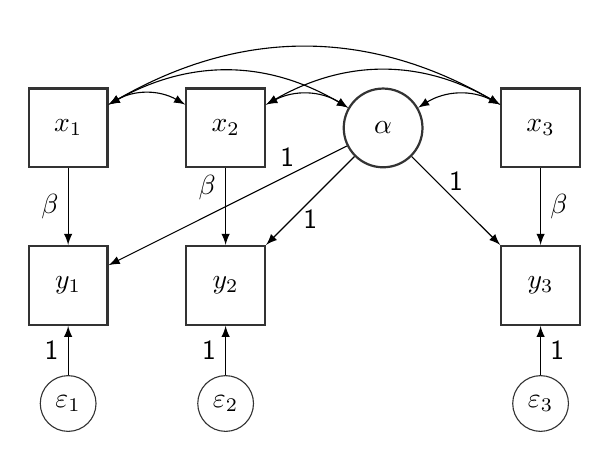
\begin{tikzpicture}
% Node styles ---
\tikzstyle{man} = [rectangle, thick, minimum size = 1cm, draw = black!80, fill = white!100, font = \sffamily] % Manifest variables
\tikzstyle{lat} = [circle, thick, minimum size = 1cm, draw = black!80, fill = white!100, font = \sffamily] % Latent variables
\tikzstyle{err} = [circle, draw = black!80, fill = white!100, font = \sffamily] % Errors 
% Edge styles
\tikzstyle{con} = [-latex, font = \sffamily] % Effects
\tikzstyle{cons} = [-latex, font = \sffamily\small] % Effects with smaller font 
\tikzstyle{cor} = [latex-latex, font = \sffamily] % Correlations
% Begin Figure ---
% Nodes 
\node at (+0.0,+0.0) [man] (x1) {$x_{1}$};
\node at (+2.0,+0.0) [man] (x2) {$x_{2}$};
\node at (+6.0,+0.0) [man] (x3) {$x_{3}$};
\node at (+4.0,+0.0) [lat] (eta) {$\alpha$};
\node at (+0.0,-2.0) [man] (y1) {$y_{1}$};
\node at (+2.0,-2.0) [man] (y2) {$y_{2}$};
\node at (+6.0,-2.0) [man] (y3) {$y_{3}$};
\node at (+0.0,-3.5) [err] (e1) {$\varepsilon_{1}$};
\node at (+2.0,-3.5) [err] (e2) {$\varepsilon_{2}$};
\node at (+6.0,-3.5) [err] (e3) {$\varepsilon_{3}$};
% Paths
\path (x1) edge [con, draw = black!100, left] node {$\beta$} (y1);
\path (x2) edge [con, draw = black!100, left, near start] node {$\beta$} (y2);
\path (x3) edge [con, draw = black!100, right] node {$\beta$} (y3);
\path (e1) edge [con, draw = black!100, left] node {1} (y1);
\path (e2) edge [con, draw = black!100, left] node {1} (y2);
\path (e3) edge [con, draw = black!100, right] node {1} (y3);
\path (eta) edge [con, draw = black!100, above, near start] node {1} (y1);
\path (eta) edge [con, draw = black!100, below] node {1} (y2);
\path (eta) edge [con, draw = black!100, above] node {1} (y3);
% correlations
\path (x1) edge [cor, bend left] node {} (x2);
\path (x1) edge [cor, bend left] node {} (eta);
\path (x1) edge [cor, bend left] node {} (x3);
\path (x2) edge [cor, bend left] node {} (eta);
\path (x2) edge [cor, bend left] node {} (x3);
\path (x3) edge [cor, bend right] node {} (eta);
\end{tikzpicture}
}
\caption{Typical three-wave FE-SEM model with contemporary effects\label{fig:fesem}}
\end{center}
\end{figure}

Let us, however, make things more concrete and take a look at a simple,
three-wave version of the typical FE-SEM using this notation (shown
graphically in Figure \ref{fig:fesem}). For that, we have the following
matrix notation (with labels on the outside of the matrices):
\begin{align}
\begin{split}
\bm{y}^{+} & = \bm{\Lambda_{y}}^{+}\bm{\eta}^{+} \\
\begin{pmatrix}
y_{1} \\
y_{2} \\
y_{3} \\
x_{1} \\
x_{2} \\
x_{3}
\end{pmatrix} & = 
\begin{blockarray}{cccccccc}
 & y_{1} & y_{2} & y_{3} & x_{1} & x_{2} & x_{3} & \alpha \\
 \begin{block}{c(ccccccc)}
 y_{1} & 1 & 0 & 0 & 0 & 0 & 0 & 0 \\
 y_{2} & 0 & 1 & 0 & 0 & 0 & 0 & 0 \\
 y_{3} & 0 & 0 & 1 & 0 & 0 & 0 & 0 \\ 
 x_{1} & 0 & 0 & 0 & 1 & 0 & 0 & 0 \\
 x_{2} & 0 & 0 & 0 & 0 & 1 & 0 & 0 \\
 x_{3} & 0 & 0 & 0 & 0 & 0 & 1 & 0 \\
 \end{block}
\end{blockarray}
\begin{pmatrix}
y_{1} \\
y_{2} \\
y_{3} \\
x_{1} \\
x_{2} \\
x_{3} \\
\alpha
\end{pmatrix},
\end{split} \label{eq:y}
\end{align} \begin{align}
\begin{split}
\bm{\eta}^{+} & = \bm{B}\bm{\eta}^{+} + \bm{\zeta}^{+} \\
\begin{pmatrix}
y_{1} \\
y_{2} \\
y_{3} \\
x_{1} \\
x_{2} \\
x_{3} \\
\alpha
\end{pmatrix} & = 
\begin{blockarray}{cccccccc}
 & y_{1} & y_{2} & y_{3} & x_{1} & x_{2} & x_{3} & \alpha \\
 \begin{block}{c(ccccccc)}
 y_{1}  & 0 & 0 & 0 & \beta & 0 & 0 & 1 \\
 y_{2}  & 0 & 0 & 0 & 0 & \beta & 0 & 1\\
 y_{3}  & 0 & 0 & 0 & 0 & 0 & \beta & 1 \\ 
 x_{1}  & 0 & 0 & 0 & 0 & 0 & 0 & 0 \\
 x_{2}  & 0 & 0 & 0 & 0 & 0 & 0 & 0 \\
 x_{3}  & 0 & 0 & 0 & 0 & 0 & 0 & 0 \\
 \alpha & 0 & 0 & 0 & 0 & 0 & 0 & 0 \\
 \end{block}
\end{blockarray}
\begin{pmatrix}
y_{1} \\
y_{2} \\
y_{3} \\
x_{1} \\
x_{2} \\
x_{3} \\
\alpha
\end{pmatrix} + 
\begin{pmatrix}
\varepsilon_{1} \\
\varepsilon_{2} \\
\varepsilon_{3} \\
x_{1} = \delta_{1} \\
x_{2} = \delta_{2} \\
x_{3} = \delta_{3} \\
\alpha = \xi \\
\end{pmatrix}. 
\end{split} \label{eq:eta}
\end{align} Notice in \(\bm{\zeta}^{+}\), for the independent variables
we could either write, for example \(x_{t}\) or \(\delta_{t}\). As
mentioned above, this is due to the model notation treating the
independent variables like dependent variables with
variances/covariances to be estimated. For the sake of simplicity, we
will ignore this subtlety and refer to the observed variable from now
on, keeping in mind that if the multivariate normality assumption holds,
the estimated statistics will likely be sufficiently close to the sample
ones for it to not make much of a difference.

Admittedly, Equations \eqref{eq:y} and \eqref{eq:eta} may not look like
much yet. We can remedy this by first putting the equation for
\(\bm{\eta}^{+}\) in reduced form, i.e., by getting rid of the dependent
variable on the r.h.s.: \begin{align}
\bm{\eta}^{+} & = \bm{B}\bm{\eta}^{+} + \bm{\zeta}^{+} \\
\bm{\eta}^{+} - \bm{B}\bm{\eta}^{+} & = \bm{\zeta}^{+} \\
(\bm{I} - \bm{B})\bm{\eta}^{+} & = \bm{\zeta}^{+} \\
\bm{\eta}^{+} & = (\bm{I} - \bm{B})^{-1}\bm{\zeta}^{+},
\end{align} where \(\bm{I}\) is the identity matrix. By substituting
this back into the equation for the observed variables we get
\(\bm{y}^{+} = \bm{\Lambda_{y}}^{+}[(\bm{I} - \bm{B})^{-1}\bm{\zeta}^{+}]\),
which works out to: \begin{align}
\begin{pmatrix} 
y_{1} \\
y_{2} \\
y_{3} \\
x_{1} \\
x_{2} \\
x_{3} \\
\end{pmatrix} & = 
\begin{pmatrix}
\alpha + \beta x_{1} + \varepsilon_{1} \\
\alpha + \beta x_{2} + \varepsilon_{2} \\
\alpha + \beta x_{3} + \varepsilon_{3} \\
x_{1} \\
x_{2} \\
x_{3}
\end{pmatrix},
\end{align} which is of course exactly what we should expect given
Equation \eqref{eq:fe}\footnote{We can use the \texttt{sympy} package in
  \texttt{python} to verify and show the steps for this and other
  examples, see the
  \href{https://github.com/henrik-andersen/FE-SEM/blob/master/sympy-doublecheck-matrixnotation.py}{supplementary
  materials} for the code.}.

\hypertarget{assumptions}{%
\subsection{Assumptions}\label{assumptions}}

What essentially differentiates an FE from an RE model is our assumption
concerning the relationship between the unobserved individual effects
and the model covariates \citep{Bollen2010}. The FE model assumes that
\(\mathop{\mathrm{\mathbb{E}}}[\alpha x_{t}] \ne 0\). As such, if we
fail to control for the correlation of the covariate and the
time-invariant part of the error, then the coefficient of interest, here
\(\beta\), will be biased. Our assumption regarding whether the
individual effects are correlated with the model covariates occurs in
\(\mathop{\mathrm{\mathbb{E}}}[\bm{\zeta}^{+}\bm{\zeta}^{+ \intercal}] = \bm{\Psi}\),
the covariance matrix of the errors \begin{align}
\bm{y}^{+}\bm{y}^{+ \intercal} & = \mathop{\mathrm{\mathbb{E}}}[(\bm{\Lambda_{y}}^{+}(\bm{I} - \bm{B})^{-1}\bm{\zeta}^{+})(\bm{\Lambda_{y}}^{+}(\bm{I} - \bm{B})^{-1}\bm{\zeta}^{+})^{\intercal}] \\
 & = \mathop{\mathrm{\mathbb{E}}}[(\bm{\Lambda_{y}}^{+}(\bm{I} - \bm{B})^{-1}\bm{\zeta}^{+})(\bm{\zeta}^{+ \intercal}(\bm{I} - \bm{B})^{-1 \intercal}\bm{\Lambda_{y}}^{+ \intercal})] \\
 & = \bm{\Lambda_{y}}^{+}(\bm{I} - \bm{B})^{-1} \mathop{\mathrm{\mathbb{E}}}[\bm{\zeta}^{+}\bm{\zeta}^{+ \intercal}] (\bm{I} - \bm{B})^{-1 \intercal}\bm{\Lambda_{y}}^{+ \intercal} \\
 & = \bm{\Lambda_{y}}^{+}(\bm{I} - \bm{B})^{-1} \bm{\Psi} (\bm{I} - \bm{B})^{-1 \intercal}\bm{\Lambda_{y}}^{+ \intercal}.
\end{align} In the case of an FE model, \(\bm{\Psi}\) will reflect our
belief that the individual effects are correlated with the model
covariates, here again for demonstration the three-wave model:
\begin{align}
\bm{\Psi} & = \mathop{\mathrm{\mathbb{E}}}
\begin{blockarray}{cccccccc}
 & \varepsilon_{1} & \varepsilon_{2} & \varepsilon_{3} & x_{1} & x_{2} & x_{3} & \alpha \\
 \begin{block}{c(ccccccc)}
 \varepsilon_{1} & \varepsilon_{1}^{2} &                     &                     &              &              &              & \\
 \varepsilon_{2} & 0                   & \varepsilon_{2}^{2} &                     &              &              &              & \\
 \varepsilon_{3} & 0                   & 0                   & \varepsilon_{3}^{2} &              &              &              & \\
 x_{1}           & 0                   & 0                   & 0                   & x_{1}^{2}    &              &              & \\
 x_{2}           & 0                   & 0                   & 0                   & x_{2}x_{1}   & x_{2}^{2}    &              & \\
 x_{3}           & 0                   & 0                   & 0                   & x_{3}x_{1}   & x_{3}x_{2}   & x_{3}^{2}    & \\
 \alpha          & 0                   & 0                   & 0                   & \alpha x_{1} & \alpha x_{2} & \alpha x_{3} & \alpha^{2} \\
 \end{block}
\end{blockarray}.
\end{align} Knowing this, we can work out the equation for the
coefficient of interest, \(\beta\). For the sake of simplicity, assume
here and throughout mean-centered variables: \begin{align}
\mathop{\mathrm{\mathrm{Cov}}}(y_{t},x_{t}) & = \mathop{\mathrm{\mathbb{E}}}[y_{t}x_{t}] \\
 & = \mathop{\mathrm{\mathbb{E}}}[(\alpha + \beta x_{t} + \varepsilon_{t})x_{t}] \\
 & = \mathop{\mathrm{\mathbb{E}}}[\alpha x_{t} + \beta x_{t}^{2} + \varepsilon_{t}x_{t}] \\
 & = \mathop{\mathrm{\mathrm{Cov}}}(\alpha, x_{t}) + \beta \mathop{\mathrm{\mathrm{Var}}}(x_{t}) \\
\hat{\beta}_{FE-SEM} & = \frac{\mathop{\mathrm{\mathrm{Cov}}}(y_{t},x_{t}) - \mathop{\mathrm{\mathrm{Cov}}}(\alpha, x_{t})}{\mathop{\mathrm{\mathrm{Var}}}(x_{t})}. 
\end{align} This should make intuitive sense. From the observed
covariance between the dependent and the independent variable, we are
partialling out the part that is due to the covariance between the
independent variable and the individual effects per unit, and then
dividing by the variance of the independent variable, as usual. For the
RE model, we assume \(\mathop{\mathrm{\mathbb{E}}}[\alpha x_{t}] = 0\)
and the equation reduces to
\(\hat{\beta}_{RE-SEM} = \mathop{\mathrm{\mathrm{Cov}}}(y_{t},x_{t})/\mathop{\mathrm{\mathrm{Var}}}(x_{t})\).
The rest of the model-implied covariance matrix results from
\(\bm{y}^{+}\bm{y}^{+ \intercal}\).

\hypertarget{fesem}{%
\section{Fixed effects in lavaan}\label{fesem}}

The package \texttt{lavaan} needs to be installed once with
\texttt{install.packages("lavaan")}. To be able to use it, we need to
load it for every new \texttt{R} session:

\singlespacing

\begin{Shaded}
\begin{Highlighting}[]
\KeywordTok{library}\NormalTok{( lavaan)}
\end{Highlighting}
\end{Shaded}

\doublespacing

For users unfamiliar with \texttt{R}, SEM analyses can be carried out
with almost no knowledge of the language. Typically, someone unfamiliar
with \texttt{R} would prepare their data using some other statistical
software, and then save the intended dataset as a \texttt{.csv},
\texttt{.xlsx}, \texttt{.dta}, \texttt{.sav}, etc. file. The user must
then import the data, preferably as a dataframe, and the rest occurs
using the \texttt{lavaan} syntax.\footnote{There are many online
  tutorials for importing data in various formats, see, for example some
  from
  \href{https://www.datacamp.com/community/tutorials/r-data-import-tutorial}{datacamp}
  or
  \href{https://www.statmethods.net/input/importingdata.html}{Quick-R},
  or any of the many posts on
  \href{https://stackoverflow.com/search?q=r+import+data}{stackoverflow}.}

Specifying the most basic fixed effects model, like the one shown in
\citet{Bollen2010} (the same model as Equation \eqref{eq:fe} but with
just one time-varying predictor) involves four components. First, we
define the latent individual effects variable using the
\texttt{=\textasciitilde{}} `measured by' or `manifested by'
\citep{R-lavaan} operator at the same time constraining the factor
loadings at each timepoint to one. I will call the latent variable
\texttt{a} to stand for \(\alpha\). Constraining all of the factor
loadings to one reflects our implicit assumption that the combined
effect of the unit-specific unobserved factors is constant over time.
This is the default behaviour of traditional POLS-based approaches to FE
that use the stacked long-format data.

\singlespacing

\begin{Shaded}
\begin{Highlighting}[]
\NormalTok{a =}\ErrorTok{~}\StringTok{ }\DecValTok{1}\OperatorTok{*}\NormalTok{y1 }\OperatorTok{+}\StringTok{ }\DecValTok{1}\OperatorTok{*}\NormalTok{y2 }\OperatorTok{+}\StringTok{ }\DecValTok{1}\OperatorTok{*}\NormalTok{y3 }\OperatorTok{+}\StringTok{ }\DecValTok{1}\OperatorTok{*}\NormalTok{y4 }\OperatorTok{+}\StringTok{ }\DecValTok{1}\OperatorTok{*}\NormalTok{y5}
\end{Highlighting}
\end{Shaded}

\doublespacing

Second, we regress the dependent variable on the independent variable
using the \texttt{\textasciitilde{}} regression operator. With stacked,
long-format data, only one regression coefficient is estimated over all
observed timepoints. To have our FE-SEM model mimic this behaviour, we
need to constrain the the estimated coefficient to equal over time. We
do so by adding the same label to the regression coefficient at every
time point. We will use the label \texttt{b} (this label was chosen
arbitrarily, we could have used any letter or string of characters) and
have it act as an equality constraint for the regression coefficient of
interest \(\beta\):

\singlespacing

\begin{Shaded}
\begin{Highlighting}[]
\NormalTok{y1 }\OperatorTok{~}\StringTok{ }\NormalTok{b}\OperatorTok{*}\NormalTok{x1}
\NormalTok{y2 }\OperatorTok{~}\StringTok{ }\NormalTok{b}\OperatorTok{*}\NormalTok{x2 }
\NormalTok{y3 }\OperatorTok{~}\StringTok{ }\NormalTok{b}\OperatorTok{*}\NormalTok{x3}
\NormalTok{y4 }\OperatorTok{~}\StringTok{ }\NormalTok{b}\OperatorTok{*}\NormalTok{x4}
\NormalTok{y5 }\OperatorTok{~}\StringTok{ }\NormalTok{b}\OperatorTok{*}\NormalTok{x5}
\end{Highlighting}
\end{Shaded}

\doublespacing

The key to a FE model, as opposed to an RE model are our assumptions
about the relatedness of our covariate and the individual effects, i.e.,
\(\mathop{\mathrm{\mathbb{E}}}[x_{t}\alpha]\). For an FE model, we want
to partial out any potential covariance between the independent variable
and the individual effects. This accounts for any linear relationship
between \(x_{t}\) and the unit-specific characteristics influencing the
dependent variable. Further, allowing unrestricted covariances between
the independent variable itself over time will not affect how the
coefficient \(\beta\) is estimated, but will have an effect on the
standard errors. To mimic the behaviour of a conventional FE model, we
allow the independent variable to be correlated with the individual
effects and itself over time. Covariances (including covariances between
a variable and itself, i.e., variances) are specified using the
\texttt{\textasciitilde{}\textasciitilde{}} operator:

\singlespacing

\begin{Shaded}
\begin{Highlighting}[]
\NormalTok{a }\OperatorTok{~}\ErrorTok{~}\StringTok{ }\NormalTok{x1 }\OperatorTok{+}\StringTok{ }\NormalTok{x2 }\OperatorTok{+}\StringTok{ }\NormalTok{x3 }\OperatorTok{+}\StringTok{ }\NormalTok{x4 }\OperatorTok{+}\StringTok{ }\NormalTok{x5}
\NormalTok{x1 }\OperatorTok{~}\ErrorTok{~}\StringTok{ }\NormalTok{x2 }\OperatorTok{+}\StringTok{ }\NormalTok{x3 }\OperatorTok{+}\StringTok{ }\NormalTok{x4 }\OperatorTok{+}\StringTok{ }\NormalTok{x5}
\NormalTok{x2 }\OperatorTok{~}\ErrorTok{~}\StringTok{ }\NormalTok{x3 }\OperatorTok{+}\StringTok{ }\NormalTok{x4 }\OperatorTok{+}\StringTok{ }\NormalTok{x5}
\NormalTok{x3 }\OperatorTok{~}\ErrorTok{~}\StringTok{ }\NormalTok{x4 }\OperatorTok{+}\StringTok{ }\NormalTok{x5}
\NormalTok{x4 }\OperatorTok{~}\ErrorTok{~}\StringTok{ }\NormalTok{x5}
\end{Highlighting}
\end{Shaded}

\doublespacing

The last component of our code involves the variances of the residuals.
This component is optional, but we can constrain the residual variances
to be equal over time to again mimic the behaviour of a conventional FE
model using POLS on stacked data. Here, again, we use labels to make
equality constraints. Because \(y_{t}\) is endogenous, the
\texttt{\textasciitilde{}\textasciitilde{}} operator specifies the
variances of \emph{residuals}, i.e., \(\varepsilon_{t}\).

\singlespacing

\begin{Shaded}
\begin{Highlighting}[]
\NormalTok{y1 }\OperatorTok{~}\ErrorTok{~}\StringTok{ }\NormalTok{e}\OperatorTok{*}\NormalTok{y1}
\NormalTok{y2 }\OperatorTok{~}\ErrorTok{~}\StringTok{ }\NormalTok{e}\OperatorTok{*}\NormalTok{y2}
\NormalTok{y3 }\OperatorTok{~}\ErrorTok{~}\StringTok{ }\NormalTok{e}\OperatorTok{*}\NormalTok{y3}
\NormalTok{y4 }\OperatorTok{~}\ErrorTok{~}\StringTok{ }\NormalTok{e}\OperatorTok{*}\NormalTok{y4}
\NormalTok{y5 }\OperatorTok{~}\ErrorTok{~}\StringTok{ }\NormalTok{e}\OperatorTok{*}\NormalTok{y5}
\end{Highlighting}
\end{Shaded}

\doublespacing

\hypertarget{ex1}{%
\section{A simulated example}\label{ex1}}

\singlespacing

\doublespacing

To demonstrate the application of FE models in SEM, a dataset can be
simulated that embodies the FE assumptions. Again, the code for data
simulation can be found in the
\href{https://github.com/henrik-andersen/FE-SEM/blob/master/simulation-code.R}{online
supplementary materials}.

To show that the latent individual effects variables represent the
\emph{combined} effect of all time-invariant characteristics, the
dependent variable will be influenced by two separate unit-specific
variables, which we can call \(\alpha_{1}\) and \(\alpha_{2}\). We will
construct the simulated data such that the independent variable is
correlated with both of the time-invariant variables. This means that
approaches that fail to account for this confounding influence, such as
POLS or RE, will be biased.

The wide-format equations for the data generating process can be
described as: \begin{align}
\bm{x_{t}} & = \bm{\alpha_{1}}\beta_{x_{t},\alpha_{1}} + \bm{\alpha_{2}}\beta_{x_{t},\alpha_{2}} + \bm{\delta_{t}}, \\
\bm{y_{t}} & = \bm{x_{t}}\beta_{y_{t},x_{t}} + \bm{\alpha_{1}}\beta_{y_{t},\alpha_{1}} + \bm{\alpha_{2}} \beta_{y_{t},\alpha_{2}} + \bm{\varepsilon_{t}} 
\end{align} where, for the sake of simplicity, \(\bm{\alpha_{1}}\),
\(\bm{\alpha_{2}}\), \(\bm{\delta_{t}}\) and \(\bm{\varepsilon_{t}}\)
are \(\sim N(0,1)\).

For the following example, a sample size of 1,000, observed over five
waves, was chosen. The unique variance of \(\bm{x}\), as well as both
the individual-effect variables is also \(\sim N(0,1)\). The coefficient
of interest, \(\beta_{y,x}\) is set to be equal to \(0.3\). A
correlation between \(\bm{x}\) and the individual effects is induced
through \(\beta_{x,\alpha_{1}} = 0.85\) and
\(\beta_{x,\alpha_{1}} = 0.50\). With the variances above set to one,
the covariances will be roughly
\(\mathop{\mathrm{\mathrm{Cov}}}(x_{t},\alpha_{1}) = 0.85\) and
\(\mathop{\mathrm{\mathrm{Cov}}}(x_{t},\alpha_{2}) = 0.5\). The
dependent variable is also influenced by the individual effects
variables with \(\beta_{y_{t},\alpha_{1}} = 0.75\) and
\(\beta_{y_{t},\alpha_{2}} = 0.45\) These values were chosen
arbitrarily.

Now, we run the FE-SEM in \texttt{lavaan}.

\singlespacing

\begin{Shaded}
\begin{Highlighting}[]
\NormalTok{fe_sem <-}\StringTok{ '}
\StringTok{# Define individual effects variable }
\StringTok{a =~ 1*y1 + 1*y2 + 1*y3 + 1*y4 + 1*y5}
\StringTok{# Regressions, constrain coefficient to be equal over time}
\StringTok{y1 ~ b*x1}
\StringTok{y2 ~ b*x2 }
\StringTok{y3 ~ b*x3}
\StringTok{y4 ~ b*x4}
\StringTok{y5 ~ b*x5}
\StringTok{# Allow unrestricted correlation between eta and covariates}
\StringTok{a ~~ x1 + x2 + x3 + x4 + x5}
\StringTok{x1 ~~ x2 + x3 + x4 + x5}
\StringTok{x2 ~~ x3 + x4 + x5}
\StringTok{x3 ~~ x4 + x5}
\StringTok{x4 ~~ x5}
\StringTok{# Constrain residual variances to be equal over time}
\StringTok{y1 ~~ e*y1}
\StringTok{y2 ~~ e*y2}
\StringTok{y3 ~~ e*y3}
\StringTok{y4 ~~ e*y4}
\StringTok{y5 ~~ e*y5}
\StringTok{'}
\NormalTok{fe_sem.fit <-}\StringTok{ }\KeywordTok{sem}\NormalTok{(}\DataTypeTok{model =}\NormalTok{ fe_sem, }
                  \DataTypeTok{data =}\NormalTok{ dfw, }
                  \DataTypeTok{estimator =} \StringTok{"ML"}\NormalTok{)}
\end{Highlighting}
\end{Shaded}

\doublespacing

\singlespacing

\doublespacing

We can get a summary of the model with \texttt{summary()}. The first
portion of the summary output gives an overview of some basic
information and fit statistics. The maximum likelihood estimator is the
default, so it did not have to be explicitly selected in the fitting
function call. Other estimators are available, including generalized and
unweighted least squares (\texttt{GLS} and \texttt{ULS}, respectively),
robust standard errors maximum likelihood (\texttt{MLM}) and several
others (see \href{https://lavaan.ugent.be/tutorial/est.html}{the lavaan
online tutorial for more}).

This part of the summary output also tells us that the analysis is based
on 1,000 observations (missings would be shown here as well if there
were any), and that the \(\chi^{2}\) statistic is 30.138 based on 32
degrees of freedom (55 observed covariances minus 1 error variance, 1
coefficient, 1 latent variable variance, 5 exogenous variable variances
and 15 covariances for \(55 - 23 = 32\) df). The p-value on the
\(\chi^{2}\) statistic is not significant with \(p =\) 0.561 which tells
us the differences between the model-implied and observed covariance
matrices are likely due to chance, and that the model fits the data well
(given how the data was generated, it would be surprising if this were
not the case). Other fit measures including typical comparative fit
indices can be requested by either adding \texttt{fit.measures\ =\ TRUE}
as a secondary argument to the \texttt{summary()} call, or by asking for
a complete list of all available fit statistics using
\texttt{lavInspect(model,\ "fit")} where \texttt{model} stands for the
name of the fitted model, in this case \texttt{fe\_sem.fit}.

\singlespacing

\begin{Shaded}
\begin{Highlighting}[]
\KeywordTok{summary}\NormalTok{(fe_sem.fit)}
\end{Highlighting}
\end{Shaded}

\begin{verbatim}
## lavaan 0.6-6 ended normally after 37 iterations
## 
##   Estimator                                         ML
##   Optimization method                           NLMINB
##   Number of free parameters                         31
##   Number of equality constraints                     8
##                                                       
##   Number of observations                          1000
##                                                       
## Model Test User Model:
##                                                       
##   Test statistic                                30.138
##   Degrees of freedom                                32
##   P-value (Chi-square)                           0.561
## 
## Parameter Estimates:
## 
##   Standard errors                             Standard
##   Information                                 Expected
##   Information saturated (h1) model          Structured
...
\end{verbatim}

\doublespacing

Next the summary output shows the measurement models for the latent
variables, if any. In this case the latent variable \texttt{a} for
\(\alpha\) is measured by each of the five observed dependent variables
with factor loadings fixed to 1.0.

\singlespacing

\begin{verbatim}
...
## Latent Variables:
##                    Estimate  Std.Err  z-value  P(>|z|)
##   a =~                                                
##     y1                1.000                           
##     y2                1.000                           
##     y3                1.000                           
##     y4                1.000                           
##     y5                1.000                           
...
\end{verbatim}

\doublespacing

The regressions are shown next. Here, because we have constrained the
regression coefficients to be equal over time (the equality constraint
label \texttt{(b)} is listed to the left of the estimates), the estimate
of \(\beta =\) 0.294 (0.016) is repeated five times. The corresponding
z- and p-values show that the coefficient is, unsurprisingly,
significant.

\singlespacing

\begin{verbatim}
...
## Regressions:
##                    Estimate  Std.Err  z-value  P(>|z|)
##   y1 ~                                                
##     x1         (b)    0.294    0.016   18.809    0.000
##   y2 ~                                                
##     x2         (b)    0.294    0.016   18.809    0.000
##   y3 ~                                                
##     x3         (b)    0.294    0.016   18.809    0.000
##   y4 ~                                                
##     x4         (b)    0.294    0.016   18.809    0.000
##   y5 ~                                                
##     x5         (b)    0.294    0.016   18.809    0.000
...
\end{verbatim}

\doublespacing

Next, the covariance estimates are listed. First, the covariances
between the latent individual effects variable and the independent
variable over time are shown, and then the covariances between the
independent variable with itself over time.

One should always take care to double-check that there are no unintended
covariances listed here. Like \texttt{Mplus}, the \texttt{lavaan}
package estimates some covariances per default, without the user
explicitly having to add them to the model syntax. For example,
covariances between latent variables are estimated per default. If one
does not wish for them to covary, it must be explicitly stated, e.g.,
with \texttt{f1\ \textasciitilde{}\textasciitilde{}\ 0*f2}, assuming the
latent variables are called \texttt{f1} and \texttt{f2}, or by
overriding the default behaviour for the entire model by adding
\texttt{orthogonal\ =\ TRUE} (which sets the correlation between all
latent variables to zero) to the fitting call.\footnote{This is at least
  the current behaviour of both the \texttt{cfa} and \texttt{sem}
  wrappers. In fact, both wrappers seem to be identical in terms of the
  default settings, see \citet{Rosseel2020}.}

\singlespacing

\begin{verbatim}
...
## Covariances:
##                    Estimate  Std.Err  z-value  P(>|z|)
##   a ~~                                                
##     x1                0.844    0.055   15.355    0.000
##     x2                0.867    0.056   15.441    0.000
##     x3                0.845    0.055   15.400    0.000
##     x4                0.822    0.053   15.455    0.000
##     x5                0.820    0.053   15.572    0.000
##   x1 ~~                                               
##     x2                0.908    0.070   12.900    0.000
##     x3                0.935    0.069   13.466    0.000
##     x4                0.921    0.067   13.661    0.000
##     x5                0.914    0.067   13.716    0.000
##   x2 ~~                                               
##     x3                0.889    0.070   12.675    0.000
##     x4                0.922    0.069   13.423    0.000
##     x5                0.889    0.068   13.165    0.000
##   x3 ~~                                               
##     x4                0.865    0.067   12.976    0.000
##     x5                0.901    0.066   13.554    0.000
##   x4 ~~                                               
##     x5                0.850    0.064   13.285    0.000
...
\end{verbatim}

\doublespacing

Finally, the variance estimates are listed. Here, we see that in order
to mimic the behaviour of a traditional FE model, the error variances
over time were specified to be equal using the equality constraint
\texttt{(e)}. Notice the \texttt{.} beside \texttt{y1}, \texttt{y2},
etc.: this indicates that the listed variance refers to an endogenous
variable, and that it is thus an error variance. In this case, these
refer to the variances of \(\varepsilon_{t}\). After that, the variances
of the exogenous variables, both observed and unobserved are listed.

\singlespacing

\begin{verbatim}
...
## Variances:
##                    Estimate  Std.Err  z-value  P(>|z|)
##    .y1         (e)    1.022    0.023   44.721    0.000
##    .y2         (e)    1.022    0.023   44.721    0.000
##    .y3         (e)    1.022    0.023   44.721    0.000
##    .y4         (e)    1.022    0.023   44.721    0.000
##    .y5         (e)    1.022    0.023   44.721    0.000
##     x1                1.986    0.089   22.361    0.000
##     x2                2.079    0.093   22.361    0.000
##     x3                1.987    0.089   22.361    0.000
##     x4                1.860    0.083   22.361    0.000
##     x5                1.814    0.081   22.361    0.000
##     a                 0.799    0.052   15.310    0.000
\end{verbatim}

\doublespacing

\hypertarget{conclusion}{%
\section{Conclusion}\label{conclusion}}

Fixed effects regression in SEM has been outlined in well-known articles
by \citep{Allison2011, Bollen2010, Teachman2001}. This article provides
a focused look at the implementation of the basic model using the
\texttt{lavaan} package in \texttt{R}. The
\href{https://github.com/henrik-andersen/FE-SEM/blob/master/extensions.pdf}{online
supplementary materials} further discuss common extensions and some
tools for evaluating and loosening model assumptions.

The benefits of FE-SEM as opposed to traditional OLS-based FE-models are
largely the same ones that apply to the SEM framework in general: for
one, SEM allows for a great deal of flexibility. For example, it is easy
to loosen model constraints as necessary. Measurement error in both the
dependent and independent variables can be dealt with using latent
variables to achieve unbiased and more efficient results. Researchers
interested in time-invariant predictors can integrate them into a hybrid
FE/RE model with ease. Further extensions, like measurement invariance
testing \citep{Schoot2012, Millsap2011, Steenkamp1998} as well as lagged
dependent variables \citep{Bollen2010, Allison2017} for example, can
also be implemented in a straightforward fashion.

The most basic FE-SEM is furthermore the basis for a variety of
currently popular extended models, such as Latent Curve Models in
general \citep{Curran2001, Bollen2004}, as well as special
implementations like the Dynamic Panel Model \citep{Allison2017}, the
Random-Intercept Cross-Lagged Panel Model \citep{Hamaker2015} and the
Latent Curve Model with Structured Residuals \citep{Curran2014}. For
this reason it is all the more important for researchers to have a good
grasp on the method of applying panel regression in SEM, and
understanding the intuition of controlling for time-invariant
confounders. This article is meant to serve as a consolidated resource
for researchers looking for concrete advise on specifying FE and more
general panel models in SEM.

\bibliographystyle{tfcad}
\bibliography{references2}




\end{document}
